% !TEX TS-program = pdflatex
% !TEX encoding = UTF-8 Unicode

% This is a simple template for a LaTeX document using the "article" class.
% See "book", "report", "letter" for other types of document.

\documentclass[11pt]{article} % use larger type; default would be 10pt

\usepackage[utf8]{inputenc} % set input encoding (not needed with XeLaTeX)
\usepackage{graphicx}
\graphicspath{ {images/} }
%%% Examples of Article customizations
% These packages are optional, depending whether you want the features they provide.
% See the LaTeX Companion or other references for full information.

%%% PAGE DIMENSIONS
\usepackage{geometry} % to change the page dimensions
\geometry{a4paper} % or letterpaper (US) or a5paper or....
% \geometry{margin=2in} % for example, change the margins to 2 inches all round
% \geometry{landscape} % set up the page for landscape
%   read geometry.pdf for detailed page layout information

\usepackage{graphicx} % support the \includegraphics command and options

% \usepackage[parfill]{parskip} % Activate to begin paragraphs with an empty line rather than an indent

%%% PACKAGES
\usepackage{booktabs} % for much better looking tables
\usepackage{array} % for better arrays (eg matrices) in maths
\usepackage{paralist} % very flexible & customisable lists (eg. enumerate/itemize, etc.)
\usepackage{verbatim} % adds environment for commenting out blocks of text & for better verbatim
\usepackage{subfig} % make it possible to include more than one captioned figure/table in a single float
% These packages are all incorporated in the memoir class to one degree or another...

%%% HEADERS & FOOTERS
\usepackage{fancyhdr} % This should be set AFTER setting up the page geometry
\pagestyle{fancy} % options: empty , plain , fancy
\renewcommand{\headrulewidth}{0pt} % customise the layout...
\lhead{}\chead{}\rhead{}
\lfoot{}\cfoot{\thepage}\rfoot{}

%%% SECTION TITLE APPEARANCE
\usepackage{sectsty}
\allsectionsfont{\sffamily\mdseries\upshape} % (See the fntguide.pdf for font help)
% (This matches ConTeXt defaults)

%%% ToC (table of contents) APPEARANCE
\usepackage[nottoc,notlof,notlot]{tocbibind} % Put the bibliography in the ToC
\usepackage[titles,subfigure]{tocloft} % Alter the style of the Table of Contents
\renewcommand{\cftsecfont}{\rmfamily\mdseries\upshape}
\renewcommand{\cftsecpagefont}{\rmfamily\mdseries\upshape} % No bold!

%%% END Article customizations

%%% The "real" document content comes below...

\title{Face Tracking for Optimized Bitrate Control in Low Delay Video Encoding}
\author{Chethan Ningaraju}
%\date{} % Activate to display a given date or no date (if empty),
         % otherwise the current date is printed 

\begin{document}
\maketitle
\clearpage
\tableofcontents
\clearpage
%%%
%%%%INTRODUCTION
%%%%
\section{Introduction}
  \subsection{Low Delay Bitrate Control}
	In recent years there is increasing demand for high quality video conferencing solutions. To address this growing need there has been constant improvement in  low delay video coding techniques. The need for extremely low end to end delay in video telephony puts additional contraints on video coding which results in compromise of video quality.

	The bitrate control module is responsible for controlling the bit-consumption of the encoder to guarantee smooth playback. Bitrate control module is not codec specific and operates independent of any chosen codec. The main purpose of the bitrate control module is to ensure efficient playback of the encoded video. Figure 1 shows the functionality the bitrate control module. It achieves this by controlling the quantization parameter using during the encoding. The decision of quantization parameter is done considering the input bitrate, framerate, input complexity (spatial and temporal activity), acceptable input delay (a measure of VBV buffer size). The module also takes the feedback from the encoder regularly to make better decision.  During the low delay video encoding, tools like bi-directional  	prediction are disabled.

\begin{figure}[h]
    \centering
    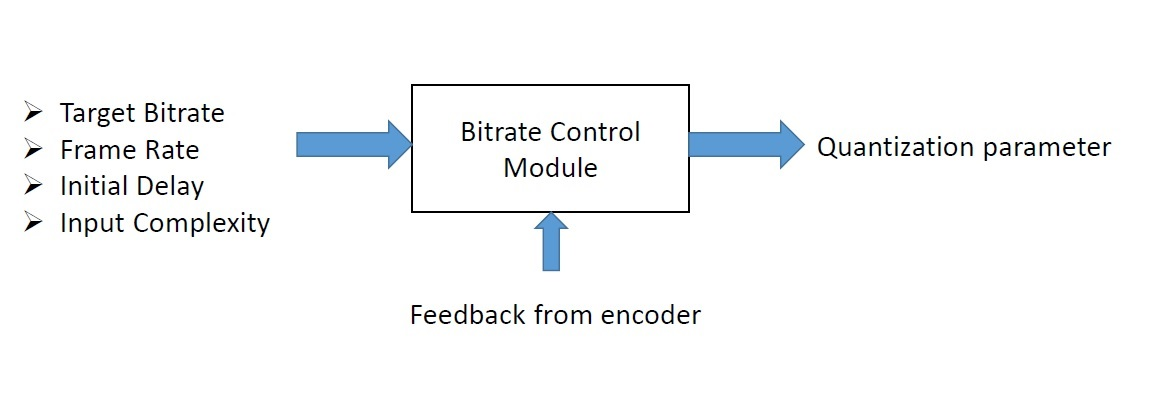
\includegraphics[scale=0.5]{RC_block}
    \caption{Bitrate Control Module Functionality}
    \label{fig:Bitrate Control Module Functionality}
\end{figure} 

  \subsection{ROI based coding}
	In conventional video coding, all regions of the frame is considered equally important. It is assumed all regions contribute equally for perceptual quality. Some video codecs use the fact that high frequency components are less important to human visual system and do you preferential coding based on spatial frequency. However, such prefential coding does not take into account the contents the frame to be encoded. 

Region of interest based coding is not a common practice in video coding because it is very hard to automatically detect important regions that contribute the most to perceptual quality. However, region of interest in video conferencing content is going to be face region predominantly. Due to recent improvements in face detection algorithms it is possible to detect face with good accuracy. The study in \cite{HighQualityROICodingForVideoConferencing} shows how boosting quality of face regions can improve the overall preceived quality of the video. This work aims to study possible ways of improving preceptual quality of the video by detecting face regions and coding it with higher quality than rest of the frame.

In order to ensure real time video communication using standard video codecs (e.g. H.264/AVC) a highly flexible bitrate-control mechanism has to be utilized. This means that the encoder's quantization parameter QP is adapted on a macroblock level in order to ensure that the maximum allowed bitcount for an encoded frame is not exceeded. In a simple approach one would try to distribute the bitrate evenly on every macroblock. Since load efficiency is of high importance it is not advisable to do multipass encoding for optimal bitrate allocation. Therefore over-allocation in one macroblock has to be compensated by under-allocation (using a higher QP) for neighboring macroblocks, regardless of the image content. However, a more intelligent allocation strategy should take the image content into account. Thus parts of the image with higher importance (e.g.faces) should be given a higher percentage of the overall bitcount which results in higher visual quality. Background regions would get a lower proportion of the bitcount.

The goal of this work is to identify the salient region of a frame, which is the face of the participant in a video conference. In a first iteration we assume ideal capture conditions so that the results of the face tracking will be directly used as side information for the H264/AVC encoder's bitrate-control. Face regions should allocate an above-average bitcount and yield a better visual quality than background regions. It is also the aim of this work to develop and extensively evaluate the strategy of uneven bitrate allocation and also to identify its limitations.

\section{Study setup}
\subsection{codec configuration}      
This work uses Citrix h264 video codec for the study. The encoder is configured in low delay mode sutiable for video conferencing. The encoder is configured to use IPPP mode with intra/key frames encoded only at the beginning of the sequence. Due to low delay there is no provision to re-encode the frame in case of buffer overflow. The frames are skipped entirely in case of buffer overflow to guarantee smoother playback by maintaning the delay constant. 

The quantization paramter is adapted at every maco-block level to meet the overall bitrate precisiely and avoid frame drops. 
\subsection{Measurements}

The most crucial aspect in this proposal is the metric used to evaluate various algorithms and choosing the best one. The goal of this proposal is to improve the quality of ROI region at the cost of non-ROI regions. The goal is to keep the bitrate constant. Since the whole approach is to measure the gain in perceptual quality, using frame level PSNR as a metric could be misleading.
In this proposal, the metric used is average PSNR of frames and it is compared with average ROI PSNR. The expectation is to see an improvement in ROI level PSNR, with degradation in PSNR of the non-ROI regions. 

In order to evaluate different algorithms, we consider different metrics. The gain of PSNR in visual ROI region and non- ROI region is measured as average PSNR of full frame and average PSNR of ROI region. This will also help in measuring the aggressiveness of an algorithm. The goal is to not make background really bad compared to the foreground.

The initial approach is to find the gain in PSNR in ROI, however finding the desirable extent of improvement in PSNR in ROI along with acceptable drop in PSNR of non-ROI is tricky. The idea here is to find the right balance between quality improvements in ROI with degradation of non-ROI region as to achieve maximum perceptual quality. For the sample video chosen, following was the PSNR measurements. The values in \ref{InitPSNR1} shows the PSNR values 
\begin{table} [h!]
\centering
\begin{tabular}{ |c|c|c| }
 \hline
Content & PSNR Avg (dB) & PSNR ROI (dB) \\
 \hline 
 Paul640x480, 250kbps & 39.22 & 37.54 \\ 
 Johny1280x720 750kbps & 40.90 & 39.20 \\  
 \hline
\end{tabular}
 \caption{Initial PSNR values}
 \label{InitPSNR1}
\end{table}

%Bibiliography and reference
\begin{thebibliography}{9}
\bibitem{HighQualityROICodingForVideoConferencing} 
Manzur Murshed and James Brown. 
\textit{High Quality Region-of-Interest Coding for Video Conferencing based Remote General Practitioner Training}. 
The Fifth International Conference on eHealth, Telemedicine, and Social Medicine.
 
\bibitem{einstein} 
Albert Einstein. 
\textit{Zur Elektrodynamik bewegter K{\"o}rper}. (German) 
[\textit{On the electrodynamics of moving bodies}]. 
Annalen der Physik, 322(10):891–921, 1905.
 
\bibitem{knuthwebsite} 
Knuth: Computers and Typesetting,
\\\texttt{http://www-cs-faculty.stanford.edu/\~{}uno/abcde.html}
\end{thebibliography}
\end{document}
